\lfoot{Autor: Daniel Melichar}
\subsubsection{Nicht relationale Datenbanken (NoSQL)}
\label{subsec:nichtrelationaleDB}

In diesem Kapitel werden ein Einblick in das Konzept von nicht-relationalen Datenbanken gegeben. Es wird nicht über die ersten Systeme gesprochen die damals dem NoSQL-Movement angehörten (Objekt-Datenbanken, XML-Datenbanken, Datenbanken für spezielle Anwendungsgebiete wie Analyse oder Streamprozessoren) diese sollten aber zumindest erwähnt werden.

\textbf{Motive und Beweggründe\newline}
Der Term \textit{NoSQL} wurde erstmalig in 1998 für eine relationale Datenbank, welche ohne der SQL-Sprache funktioniert, verwendet\cite{MELD.CH2-noSQL.firstSQLNaming}. Der Term wurde dann wieder in über die Jahre von verschiedensten Leuten aufgenommen. Unglücklicherweise gab es keine definitive Beschränkung für welche Datenbanksysteme zum NoSQL-Movement gehören. Durch den Blogger und Rackspace Mitarbeiter, Eric Evans, ist der Term ganz besonders bekannt geworden – er sagte hierzu: \cite[\textit{“the whole point of seeking alternatives is that you need to solve a problem that relational databases are a bad fit for”}]{MELD.CH2-noSQL.whatsInAName}. NoSQL Datenbanken wurden hauptsächlich von Großkonzernen für den Eigenbedarf entwickelt (Amazon’s Dynamo, Google’s BigTable, LinkedIn’s Voldemort, Facebook’s Cassandra, Yahoo!’s PNUTS). Diese Großkonzerne haben den relationalen Ansatz nicht komplett verworfen, sie fanden lediglich, dass das Model nicht den Anforderungen entspricht\cite{MELD.CH2-noSQL.capTheoremComp}.

Das bekannte IT und Technologie Magazine \textit{Computerworld} hat in 2009 bei einer NoSQL Konferenz in San Franciso die dort vorhanden Developer befragt wieso NoSQL gegenüber relationalen Datenbanken im Vorteil liegt\cite{MELD.CH2-noSQL.whyItsBetter}.

Die folgenden Erklärungen wurden von den Entwicklern gemacht.
\begin{itemize}
	\item \textbf{Unnötige Komplexität wird vermieden}\newline
	 Relationale Datenbanken verfügen über eine große Anzahl an Features und strikter Daten Konsistenz Vorschriften. Jedoch kann diese Anzahl an Features und die Anbindung an das ACID-Model zu viel für spezifische Anwendungsfälle sein. Zum Beispiel ist die Überprüfung von Session Daten die Mehrmals als Kopie abgespeichert sind nicht notwendig.

	\item \textbf{Hohe Verarbeitungsmenge}\newline
	 Manche NoSQL Datenbanken verfügen über eine weitaus größere 	Verarbeitungsmenge. So wird bei dem column-store Hypertable, welches die Ziele von Google’s BigTable verfolgt, erlaubt es bis zu einer Millionen Datensätze pro Tag zu speichern. Ein weiteres Beispiel ist Google’s BigTable selbst; es kann bis zu 20 Petabyte pro Tag verarbeiten.

	\item \textbf{Horizontale Skalierbarkeit und geringe Hardware requirements}\newline
	 Im Vergleich mit relationalen DBMS sind die meisten NoSQL Datenbanken so konzipiert um horizontale Skalierung möglichst einfach durchzuführen. Horizontale Skalierung bedeutet prinzipiell mehr Server, oder im allgemeinen Verarbeitungsmachinen, in den Pool der Ressourcen hinzu zu fügen. Es gibt zwar auch eine äquivalente Verbesserungsmöglichkeitne für RDBMS, das so genannte \textit{sharding}, dies ist oft aber weit aus komplizierter als bei NoSQL. Zum Beispiel gibt es bei der Bekannten NoSQL Datenbank \textit{MongoDB} eine automatische Version der Sklaierung.

	\item \textbf{Object-Relational Mapping wird vermieden}\newline
	 Auch hier verwenden die meisten NoSQL Datenbanken eine Struktur zur Speicherung der Daten die entweder sehr Simple oder sehr Ähnlich zu jenen sind die auch bei Objekt-Orientierten-Programmiersprachen aufzufinden sind. Hierfür ist dann kein ressourcenintensives Object-Relational Mapping notwendig.
\end{itemize}

Zu diesem Bericht gab es dann auch einen Blog post von Nati Shalom, CTO und Gründer von GigaSpaces. Er hat die folgenden weiteren Punkte für die NoSQL-Bewegung aufgestellt\cite{MELD.CH2-noSQL.natiShalomlol}.

\begin{itemize}
	\item \textbf{Komplexität und benötigter Aufwand bei Datenbank Clustern}\newline
	 Er meint, dass NoSQL Datenbanken auf eine Art und Weise entwickelt worden sind, die das erstellen von Clustern sehr einfach macht. Unter anderem spielt hier auch das bereits angesprochene Skalieren auf horizontaler Ebene eine große Rolle.
	
	\item \textbf{Kompromiss zwischen Performance und Verlässlichkeit}\newline
	 Shalom behauptet außerdem, dass verschiedene Szenarien gibt, in welchen Applikationen den Fokus auf Performance legen und nicht auf Verlässlichkeit. Ein gutes Beispiel für dieses Szenario sind die Daten von HTTP Sessions – diese müssen zwischen vielen Web Servern geschickt werden, löschen sich aber dann sobald der User sich abmeldet.

	\item \textbf{Cloud Computing}\newline
	 Hier werden sehr oft NoSQL Lösungen verwendet, da dass Limit der Skalierbarkeit sehr hoch, bis sogar unendlich ist, es wenig administrative Tätigkeiten im Umgang mit NoSQL gibt, es viele NoSQL Datenbanken gibt die spezifisch für Datawarehousing entiwckelt worden sind, uvm.
\end{itemize}

\textbf{Techniken und Konzepte\newline}
\htab\textbf{Das CAP-Theorem\newline}
Das von Eric Brewer im Jahre 2000 entwickelte CAP-Theorem ist heutzutage in vielen Web-Unternehmen (z.B. Amazon) aber auch in der NoSQL Community aufzufinden\cite{MELD.CH2-noSQL.capTheorem}. Der CAP Akronym steht für:

\begin{itemize}
	\item \textit{Consistency:} Ob und wie ein System in den konsistenten Zustand, nach Ausführung einer Operation, zurück gelangt. Ein verteiltes System wird im Normalfall als Konsistent bezeichnet, wenn alle lesenden Teile das selbe Resultat aus dem geteilten Informationspool bekommen.

	\item \textit{Availability:} Hierbei ist vor allem auf das Design und Umsetzung eines Systems zu achten. Es sollte so entwickelt sein, dass bei Ausfall eines Servers in einem Cluster immer noch die selben Operationen durchgeführt werden können.

	\item \textit{Partition Tolerance:} Anders als bei Availability geht es hier meistens um Netzwerk Partitionen und die Möglichkeit weiter Operationen durchzuführen, wenn zwei Netzwerke im System nicht miteinander kommunizieren können.
\end{itemize}

 Brewer behauptet, dass man nur zwei von diesen drei Eigenschaften in einem \textit{shared-data system} haben kann\cite{MELD.CH2-noSQL.capTheorem}. In seiner Präsentation hat er über die Vor- und Nachteile von ACID und BASE Systemen (siehe nächsten Paragraphen) geredet und einige Entscheidungskriterien vorgestellt um sich für eine der beiden Modelle zu entscheiden: wenn ein System, oder Teile eines Systems, konsistent und Partition-Tolerant sein müssen, sind ACID Eigenschaften benötigt; wenn Verfügbarkeit und Partition-Tolerants benötigt werden, sollte das System mittels BASE Eigenschaften erstellt werden. Anhand folgender Tabelle, welche direkt aus seiner Präsentation genommen wurde, lässt es sich am besten veranschaulichen.

\begin{table}[!htb]
\centering
\begin{tabular}{|l|l|l|}
\hline
\multicolumn{1}{|c|}{\textbf{Choice}} & \multicolumn{1}{c|}{\textbf{Traits}} & \multicolumn{1}{c|}{\textbf{Examples}} \\ \hline
Consistence + Availability & \begin{tabular}[c]{@{}l@{}}2-phase-commit\\ cache-validation protocols\end{tabular} & \begin{tabular}[c]{@{}l@{}}Single-site databases\\ Cluster databases\\ LDAP\\ xFS file system\end{tabular} \\ \hline
Consistency + Partition tolerance & \begin{tabular}[c]{@{}l@{}}Pessimistic locking\\ Make minority partions unavailable\end{tabular} & \begin{tabular}[c]{@{}l@{}}Distributed databases\\ Distributed locking\\ Majority protocols\end{tabular} \\ \hline
Availability   + Partition tolerance & \begin{tabular}[c]{@{}l@{}}expirations/leases\\ Conflict resolution\\ Optimistic\end{tabular} & \begin{tabular}[c]{@{}l@{}}Coda\\ Web caching\\ DNS\end{tabular} \\ \hline
\end{tabular}
\caption{CAP-Theorem – Alternatives, Traits, Examples \cite{MELD.CH2-noSQL.capTheorem}}
\end{table}

Grundsätzlich kann man sagen, dass bei relationalen Datenbanken weniger Availability herscht als bei der NoSQL Variante. Beide Systeme verfügen jedoch über Partition Tolerance\cite{MELD.CH2-noSQL.capTheoremComp}

\begin{figure}[!htb]\centering
	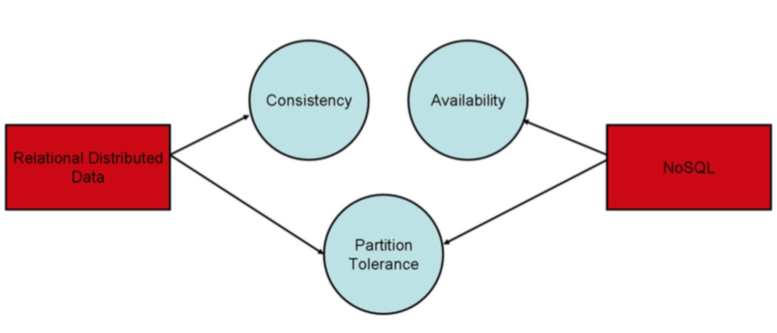
\includegraphics[width=0.8\textwidth]{images/capTheorem}
	\caption{CAP-Theorem bei RDBMS und NoSQL\cite{MELD.CH2-noSQL.capTheoremComp}}
\end{figure}

\textbf{ACID vs BASE\newline}
Das Internet erzeugt Tag für Tag für eine enorme Menge an Daten welche verarbeitet, analysiert und bereitgestellt werden müssen. Die Applikationen und Service in diesem Bereich müssen den individuellen Bedarf an Performance, Zuverlässigkeit, Betriebsbereitschaft, und Konsistenz feststellen. Wie bereits beim CAP-Theorem beschrieben können diese Applikationen und Service nur zwei Optionen von Consistency, Availability, und Partition Tolerance, genommen werden. Immer mehr Applikationen und Service bevorzugen die Option von Availability und Partition Tolerance und vernachlässigen somit die strikte Toleranz. Diese Eigenschaften sind schwer mit dem ACID Model zu erreich, jedoch wurde dafür das BASE Model entwickelt. Es gibt kein Model das besser ist, man muss das richtige Model für seine Bedürfnisse wählen.

Das Akronym BASE steht für folgende Eigenschaften
\begin{itemize}
	\item Basically Available
	\item Soft-state
	\item Eventual consistency
\end{itemize}

Brewer stellt den Vergleich zwischen ACID und BASE mit der Darstellung, welche man in der Tabelle sehen kann. Es ist jedoch zu beachten das diese beiden Konzepte sich nicht aufheben sollen, sondern ein großes Spektrum an Möglichkeiten bieten sollen. 

\begin{table}[!htb]
\centering
\label{acidvsbaseTable}
\begin{tabular}{|l|l|}
\hline
\multicolumn{1}{|c|}{\textbf{ACID}} & \multicolumn{1}{c|}{\textbf{BASE}} \\ \hline
\begin{tabular}[c]{@{}l@{}}Strong consistency \\ Isolation \\ Focus on “commit” \\ Nested transactions \\ Availability? \\ Conservative (pessimistic) \\ Difficult evolution (e.g. schema)\end{tabular} & \begin{tabular}[c]{@{}l@{}}Weak consistency – stale data OK \\ Availability first\\ Best effort \\ Approximate answers OK \\ Aggressive (optimistic)\\ Simpler!\\ Faster \\ Easier evolution\end{tabular} \\ \hline
\end{tabular}
\caption{ACID vs BASE \cite{MELD.CH2-noSQL.capTheorem}}
\end{table}

\textbf{Partitionierung\newline}
Ab einer gewissen Menge an Daten werden die benötigten Ressourcen über die Kapazität einer einzelnen Maschine hinaus laufen. In diesem Fall müssen die Daten über mehrere Maschinen aufgeteilt werden – das nennt man \textit{Partitioning}. Hierbei gilt es auch zu beachten, dass  das System weiterhin funktionsfähig sein muss, wenn einer dieser Maschinen ausfällt. Es sollte auch beachtet werden, dass die Last der Ressourcen auf alle Server aufgeteilt ist (\textit{load balancing}).

Bei NoSQL Datenbanken gibt es hierfür verschiedene Konzepte um die Best möglichen Ergebnisse zu erhalten.

\begin{description}
	\item[Memory Caches] können als separate Zwischenspeicher (z.B. RAM) Datenbanken geshene werden. Hierbei werden die am meist gebrauchten Daten mit einer hohen Frequenz in den Memory gespeichert und somit eine Art von Caching entwickelt. In den meisten Fällen hollt man sich dann die Daten über eine API und einen speziellen Key.

	\item[Clustering] von Datenbanken ist eine weitere Möglichkeit. Hierbei ist es vor allem sehr wichtig, dass der Verwendet der Applikaion gar nicht mit bekommt mit wie vielen Servern er kommuniziert.

	\item[Trennung von Read und Write] bedeutet, dass es spezifische Server gibt die nur Schreiben, bzw. nur Lesen dürfen. Durch die asynchrone Verarbeitung der Daten gibt es beinahe keinen lag zwischen den Servern und durch Replikation der Daten (Mehrfachspeicherung) ist es auch schwierig die Daten zu verlieren

	\item[Sharding] ist ein Prinzip in welchem die Daten so gespeichert sind, dass die Antworten auf die Requests nahe zusammenliegen selbst auf einem einzigen Server. Auch hier spielt bei mehreren Servern die Verteilung eine große Rolle. Die konkrete Umsetzung von Sharding ist eine mathematisch sehr komplizierte und würde den Rahmen sprengen.
\end{description}

\textbf{Kritik\newline}
Selbstverständlich gibt es nicht nur positive Dinge über NoSQL. Auch nicht relationale Systeme haben einige Punkte in welchen es noch Verbesserungsbedarf gibt \cite{MELD.CH2-noSQL.sqlvsnosql}. 

\begin{itemize}
	\item \textbf{Vortschritt\\}
	Relationale Datenbanken existierten schon um einige Jahre länger als die NoSQL Variante. Die Zielsetzung von RDBMS ist es stabil und verlässlich zu sein - was teilweise auch bedeutet, dass es wenige neue Innovationen gibt. Hingegen gibt es noch einige NoSQL Datenbanksysteme die ein Basis Feature-Set entwickeln müssen.

	\item \textbf{Support\\}
	Auch hier spielt die etwas längere Lebensdauer von RDBMS eine große Rolle. Solche Namen wie \textit{MySQL, PostgreSQL, Microsoft SQL Server} sind sehr bekannt in der IT Welt. Die Entwickler dieser Systeme setzen auch auf einen guten Support, wobei dieser oft nur for Enterprise Editions zur Verfügung steht. Hingegen sind die meisten NoSQL Datenbanken Open Source, und haben daher meist nur Community Support. Ob dieser Ansatz gut oder schlecht ist eine Ansichtssache von Open Source Projekten.

	\item \textbf{Administration\\}
	Der wahrscheinlich größte negative Aspekt von NoSQL ist die eigentliche Administration. Es wird zwar oft gesagt, dass NoSQL keine administrativen Tätigkeiten benötigt, in den meisten Fällen muss aber trotzdem hin und wieder an der Datenbank gefeilt werden. Bei relationalen Datenbanken gibt es durch Einsatz von Persmissions, Rollen, und durch das ACID-Model weit aus einfache administrative Möglichkeiten.

	\item \textbf{Fehlende Standardisierung\\}
	Bei relationalen Datenbanken gibt es zwar auch eine einheitliche Programmiersprache die prinzipiell für alle DBMS funktioniert, aber auch hier gibt es verschiedene Dialekte. Bei NoSQL Datenbanken ist es dem Entwickler überlassen wie er mit der Datenbank kommunizieren will. In den meisten Fällen wird JavScript verwendet, es kann aber auch eine eigene, komplett neue Programmier- oder Skriptsprache sein.
\end{itemize}

\textbf{Klassifikation von NoSQL Datenbanken\newline}
Zum Zeitpunkt der Erstellung dieses Dokuments gibt es weit über zweihundert NoSQL Datenbanken\cite{MELD.CH2-noSQL.listOfNoSQLDB}. All diese Datenbanken können in vier Kategorien eingeteilt werden:

\begin{itemize}
	\item Key-Value Stores
	\item Column-Oriented Databases
	\item Document Databases
	\item Graph Stores
\end{itemize}

Für eine detailierte Beschreibung, Anwendungsfälle, und Vergleiche, siehe Sektion \ref{subsec:dbms}

\clearpage